\graphicspath{{Billeder/}}

\chapter{Design}
\section{Formål}
Formålet med denne opgave er at lave et sytem der kan monitorere og præsentere flytraffik over et givent område. Der vil også blive kigget på om flyene i området flyver for tæt. Informationer om flight-tracks vil blive indhentet fra en TransponderReceiver, givet i strings. Dernæst objektifiseres disse strings, og objekterne præsenteres i en konsol. 
Hele systemet vil blive testet ved hjælp af både unit tests samt integrationstests.


\section{Design}
Link til Github: \url{https://github.com/TeamTyve/ATM} \newline \newline 
Der er i opgaven givet en .dll fil der benyttes til at indhente flight-tracks og præsentere disse i strings. Der implementeres derfor en Track Objectification Service, som benyttes til at objektifisere de indhentede strings. \tabularnewline
Formålet med at få objektifiseret disse strings, er at man får gjort de indhentede strings meget mere overskuelige når de omdannes til objekter, samt at det bliver muligt at arbejde på disse objekter. \newline
Objekterne er fly, som består af henholdsvis et tag (navnet på flyet), x- og y-koordianter, højde i luften, hastighed, retning i grader samt et timestamp. \newline

Når flyene er blevet objektifiseret vil der blive checket for nogle forskellige ting. \tabularnewline
Først vil der blive checket for, om et fly er i et givent område - kaldet AirSpace. Hvis flyet er i AirSpace, vil flyets informationer blive udskrevet til konsollen.
Dernæst vil der blive checket på om de fly, der er i det givne område, flyver for tæt på hinanden. Hvis dette skulle være tilfældet, vil der udskrives en advarsel på konsollen, omkring hvilke fly der flyver for tæt på hinanden, samt hvad tid advarslen fremkom. \newline

\textbf{Klassediagram - Vedhæftet som bilag bagerst i dokumentet} \\
På klassediagrammet ses hvordan systemet er opbygget. \tabularnewline
Det ses hvordan klassen TrackObservationSystem (TOS) er "hovedmodulet", der er forbundet til de andre klasser.
Klassen "TrackingSystem" benyttes til at modtage en TransponderReceiver fra .dll filen. Denne TransponderReceiver overføres herefter til TOS.
TOS er også koblet til TrackRepository der persisterer Tracks. TrackRepository benyttes til at udregne ting som hastighed, retning, distance etc. Det er denne klasse som i sidste ende objektifiserer de strings der bliver indhendtet fra TrackingSystem og over i TOS.

Klassen "AirSpace" benyttes til at tjekke om et fly er inde i AirSpace.

Derudover indeholder systemet også klasser som Seperation, SeperationAlertRepository samt SeperationAlert. Disse klasser benyttes til at tjekke om de fly, der er inde i AirSpace, flyver for tæt på hinanden. 

Klasserne Output, LogHelper, ConsoleLogger og EventLogger er allt klasser der er med til at få printet dataen til konsollen. 

Grunden til at der findes både ConsoleLogger samt EventLogger, er at EventLogger persisterer de events, der kommer, ned i en fil og ConsoleLoggeren skriver dataen ud på konsollen. \newline

\textbf{Sekvensdiagram - Vedhæftet som bilag bagerst i dokumentet} \\
På sekvensdiagrammet ses det hvordan klasserne interagerer med hinanden. \tabularnewline
Det ses her hvordan TrackingSystem starter med at modtage en ITransponderReceiver fra klassen TransponderrReceiver der ligger i .dll filen. \tabularnewline
Herefter oprettes et nyt TrackObservationSystem der medtager denne ITransponderReceiver som parameter.\tabularnewline
Nu indhendtes der dermed data om indkommende fly. I sekvensdiagrammet gåes der herefter ind i en "alt". \tabularnewline
Så snart der er noget TransponderData klar vil denne data bearbejdes - Dataen, som indhendtes i strings, vil blive objektifiseret og der vil blive checket om de er i Airspace, samt om de flyver for tæt på andre fly inde i AirSpace.
Disse data vil blive udskrevet hvis ConsoleOut er lig med true vil flyene i AirSpace blive udskrevet til konsollen.

Der er mulighed for at der sker et SeperationEvent. \tabularnewline
Hvis flyene er for tæt på hinanden ved check via funktionen "CheckSeperation()" vil der blive raiset et SeperationEvent. 
Dette vil resultere i, som der også ses på diagrammet, at en warning udskrives i konsollen.


\section{Resultater}
Link til Jenkins - Coverage: \url{http://ci3.ase.au.dk:8080/job/TeamTyveATMCoverage/} \\
Som det ses på nedenstående billede virker systemet som forventet. De tracks der ligger inde i AirSpace bliver udskrevet på konsollen med alle de ønskede informationer.

De warnings der kommer, når to fly flyver for tæt, bliver udskrevet nederst i konsollen.\newline

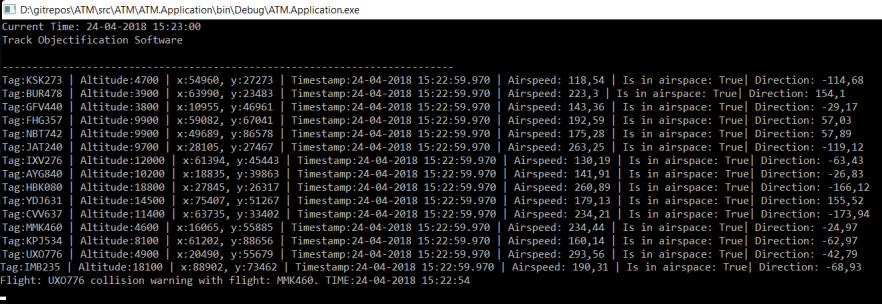
\includegraphics[scale=0.55]{1.PNG}





